\epigraph{God does not play dice --- but the butterfly flutters at all scales.}{}

\section{Determinism in Principle}


\begin{figure}[htbp]
\centering
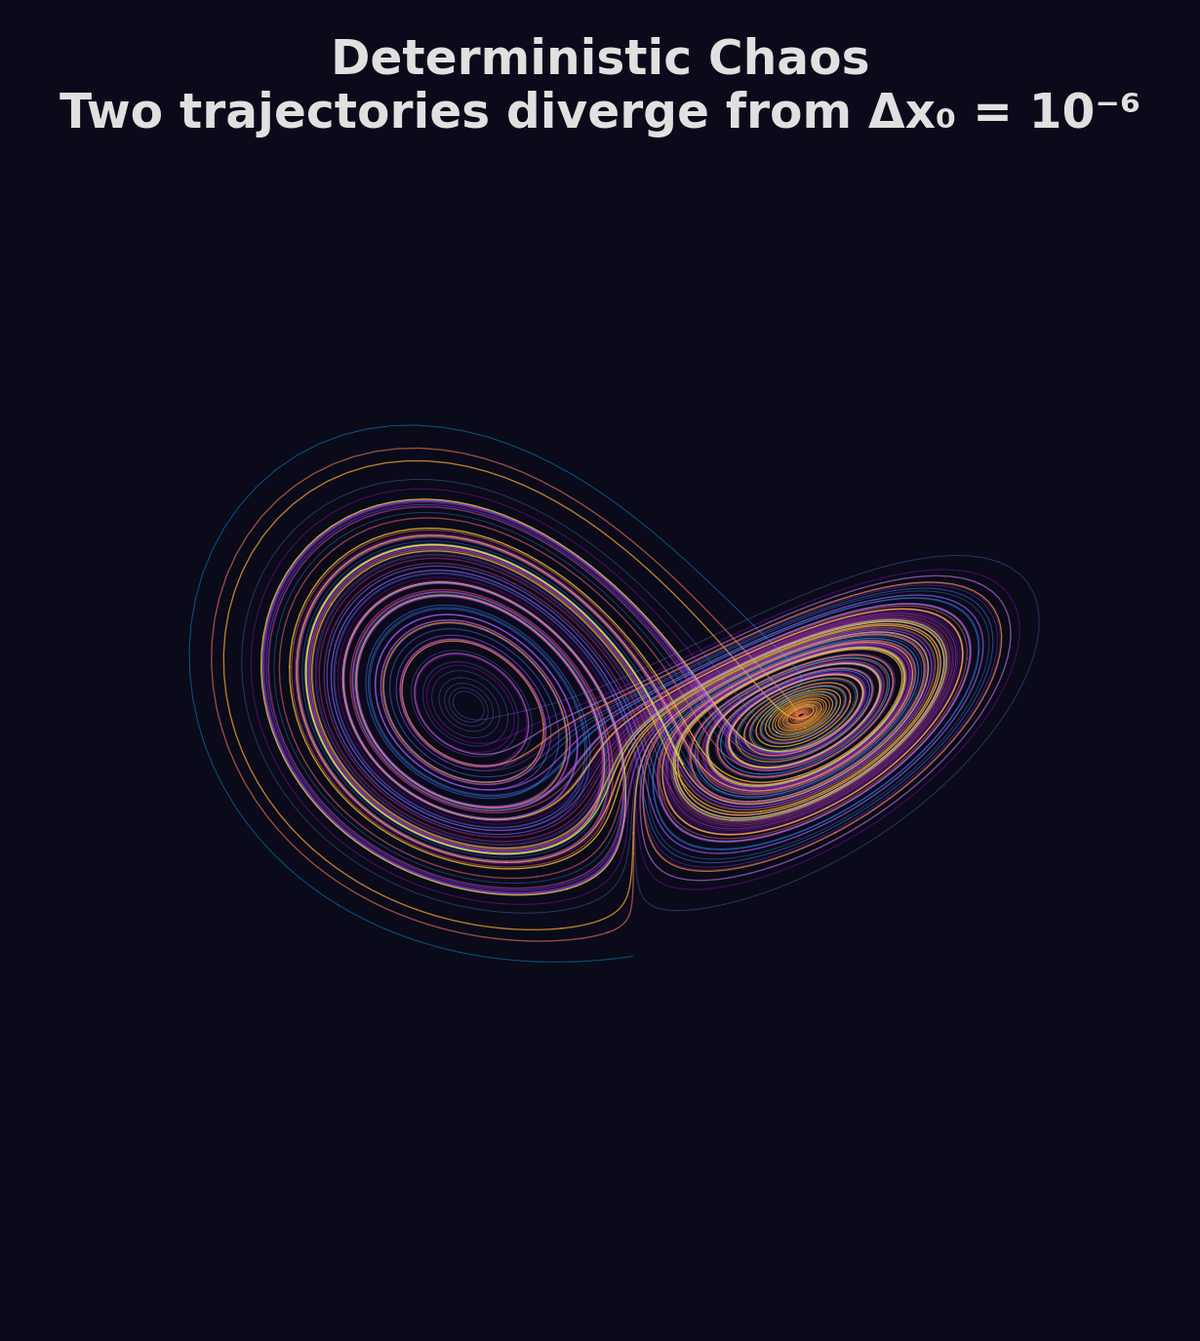
\includegraphics[width=0.85\textwidth]{img/ch12_butterfly.png}
\caption{Deterministic chaos: the Lorenz attractor as an analogy for the fractal butterfly effect.}
\end{figure}
In T0 everything is determined in principle. The time field~$\Tfield$ evolves fully causally. There is no fundamental randomness, no dice throw of God, no irreducible noise in the foundation of nature.

What appears as quantum randomness --- radioactive decay, the outcome of a spin measurement, the position of an electron in the double-slit experiment --- is deterministic time-field dynamics with \emph{practically unpredictable} outcomes.

\section{Why Only Probabilities Are Calculable}

If nature is deterministic, why do probability calculations work so well? The answer lies in the fractal, recursive complexity of the brain-fold torus.

Every measurement disturbs the system it measures. The system reacts to the disturbance. The disturbance reacts to the reaction. An infinite feedback loop arises. The fractal structure --- $\Df = 3 - \xsi$ --- generates new interaction layers at every scale. The number of relevant degrees of freedom grows faster than any computable function.

An analogy: the weather is a fully deterministic system. The Navier-Stokes equations describe exactly how the atmosphere evolves. And yet an exact weather forecast is impossible after just a few days --- the butterfly effect ensures that the tiniest perturbations grow exponentially.

In the torus this effect is raised \emph{fractally across all scales}. It is as if the butterfly effect acted not only at the weather scale but simultaneously at the molecular, atomic, and subatomic scales --- and all these scales were coupled to one another.

\section{The Born Rule as an Emergent Law}

This is why the probability description works. The Born rule of quantum mechanics --- $P = |\psi|^2$ --- is not fundamental (cf.\ \href{https://github.com/jpascher/T0-Time-Mass-Duality/blob/main/2/pdf/073_QM-testen_De.pdf}{Doc.~073}, \href{https://github.com/jpascher/T0-Time-Mass-Duality/blob/main/2/pdf/074_NoGo_De.pdf}{074}). It is \emph{emergent}: a statistical law over a deterministic substrate. Just as thermodynamics emerges from deterministic Newtonian mechanics, quantum statistics emerges from the deterministic T0 dynamics.

The probability description works not because nature is random. It works because the deterministic complexity exceeds our computational capacity --- and any principally possible computational capacity.

\begin{kerngedanke}
T0 unites the seemingly irreconcilable: complete determinism with practical unpredictability. Nature is computable --- but not by us, and not by any finite computer. The Born rule is the best compass in a labyrinth too complex for an exact map.
\end{kerngedanke}
